\chapter{HDF5 C++ Interface}
%\section{Example Section}
%\subsection{Example Subsection}
%\subsubsection{Example Subsubsection}
%\paragraph{Example Paragraph}
%\subparagraph{Example Subparagraph}
\section{Overview}
The acronym HDF stands for hierarchical data format meaning this binary format is allowing to structure the internal objects after the users demand. This structure is quite similar to a file system where data is ordered with folders and sub-folders. For more detailed information see the official C \cite{hdf5cdoc} and C++ \cite{hdf5cppdoc} documentation. The reason why also the C documentation is very important is based on the fact that the C++ implementation is mostly a nice wrapper based on the C implementation. For the exact dependence see table \ref{table:corrs}.
\begin{figure}[ht!]
\centering
\begin{tabular}{|l|l|}
\hline
HDF5 C APIs&C++ Classes\\
\hline
Attribute Interface (H5A)&Attribute\\
Datasets Interface (H5D)&DataSet\\
Error Interface (H5E)&Exception\\
File Interface (H5F)&H5File\\
Group Interface(H5G)&Group\\
Identifier Interface (H5I)&IdComponent\\
Property List Interface (H5P)&PropList and subclasses\\
Dataspace Interface (H5S)&DataSpace\\
Datatype Interface (H5T)&DataType and subclasses\\
\hline
\end{tabular}
\caption{Table of correspondence between C and C++}
\label{table:corrs}
\end{figure}
To use the C++ language features to its most capabilities inheritance is used. This allows reuse of functions, objects and properties over many hierarchy layers. This enforces a strict dependence when sharing or creating objects. To have an overview on the hierarchy look at figure \ref{graph:hierarchy}.

\begin{figure}[ht!]
\centering
\resizebox{\textwidth}{!}{
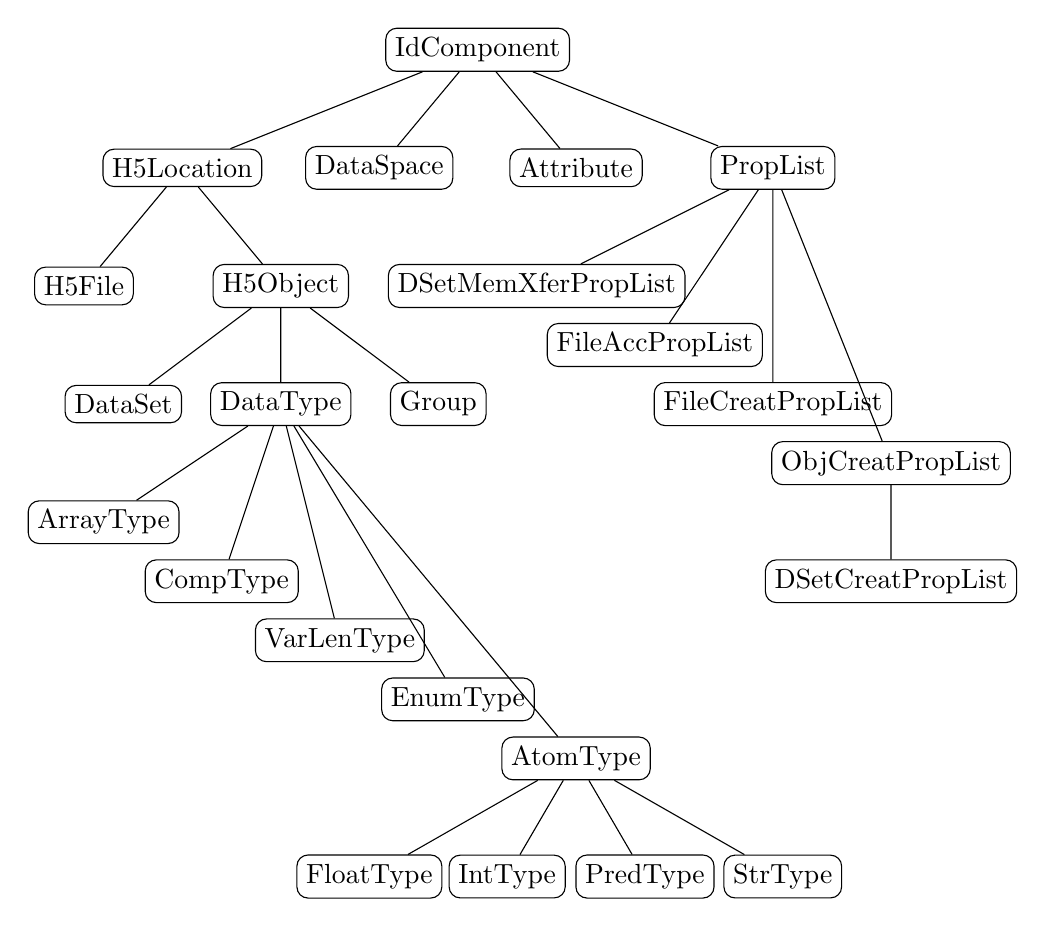
\begin{tikzpicture}[
baseline,
every node/.style = {shape=rectangle, rounded corners, draw, align=center},
]]
  \node {IdComponent}
    child[xshift=-1.5cm]
    {
        node{H5Location}
    	child[xshift=-0.5cm]{node{H5File}}
    	child[xshift=0.5cm]
    		{
    		node{H5Object}
    		child[xshift=-0.5cm]{node{DataSet}}
    		child{
    			node{DataType}
    			child[xshift=0.75cm]{node{ArrayType}}
    			child[xshift=0.75cm,yshift=-0.75cm]{node{CompType}}
    			child[xshift=0.75cm,yshift=-1.5cm]{node{VarLenType}}
    			child[xshift=0.75cm,yshift=-2.25cm]{node{EnumType}}
    			child[xshift=0.75cm,yshift=-3.0cm]
    				{
    				node{AtomType}
    				child[xshift=-0.375cm]{node{FloatType}}
    				child[xshift=-0.125cm]{node{IntType}}
    				child[xshift=0.125cm]{node{PredType}}
    				child[xshift=0.375cm]{node{StrType}} 
    				}
    			}
    		child[xshift=0.5cm]{node{Group}}
    		}
 	}
    child[xshift=-0.5cm]{node{DataSpace}}
    child[xshift=0.5cm]{node{Attribute}}
    child[xshift=1.5cm]{
    	node{PropList}
    	child[xshift=-0.75cm]{node{DSetMemXferPropList}}
    	child[xshift=-0.75cm,yshift=-0.75cm]{node{FileAccPropList}}
    	child[xshift=-0.75cm,yshift=-1.5cm]{node{FileCreatPropList}}
    	child[xshift=-0.75cm,yshift=-2.25cm]{
    		node{ObjCreatPropList}
    		child{node{DSetCreatPropList}}
    		}
    		};
\end{tikzpicture}
}
\caption{Depiction of derivation hierarchy}
\label{graph:hierarchy}
\end{figure}

As stated in the background this project is about the simulation of \textit{Hagedorn} wavepackets over a fixed time horizon. To keep track and possibly reproduce the results the wavepackets have to be saved in every time step $\Delta t$ of the simulation. This has to be achieved with the classes shown in figure \ref{graph:hierarchy}. To understand the functionality of these classes they will be explained in the following sections.

\section{Internal types and states}
\label{seq:internaltypes}
An interface in general has supported objects and functions. These functions also have preconditions and postconditions whereas objects have valid states. In case of the HDF5 library when these are not fulfilled an exception is thrown which could abort or interrupt the program execution. Therefore it is important to always use valid objects and function calls. There are two noteworthy types which are also used the most. These are \texttt{hsize\_t} and \texttt{H5std\_string}. Variable of type \texttt{hsize\_t} represent native multiple-precision integer. This type substitutes the C++ internal \texttt{int} data type. The \texttt{H5std\_string} type is just an alias for the \texttt{std::string} data type from the standard library. Internal valid states are represented in only uppercase letters and with the C prefix as in table \ref{table:corrs}. For example a valid property list state is \texttt{H5P\_DEFAULT}.

\section{H5File}
As the name already suggest this class is used to manage the binary file object. When a \textit{H5File} is default constructed it also allocates a default \textit{Group} root named "/". To construct a \textit{H5File} a minimal number of two arguments is needed. The two additional optional arguments are a \textit{FileCreatPropList} and a \textit{FileAccPropList} which would allow further specification. These would be creation and access properties as suggested by the names. In case of this project they are not needed and the \texttt{H5P\_DEFAULT} is sufficient. For the first mandatory argument, which is the filename, a \texttt{H5std\_string} or as discussed before a string required. The second mandatory argument defines the type of creation which at default has two valid values. These possible values are \textit{H5F\_ACC\_TRUNC} and \textit{H5F\_ACC\_EXCL} which are mutually exclusive. The former truncates the file meaning if it already exists erase all data previously stored in the file. The latter fails if the file already exists under the specified name which ends in an exception. It is advised to work with \textit{H5F\_ACC\_TRUNC} because it is simpler and thus errors will less frequently occur.

\section{Group}
\label{seq:group}
As previously mentioned it is a hierarchical data format. The hierarchy gets implement through the usage of \textit{Groups}. In case of a \textit{Hagedorn} wavepackets and its corresponding energies the structure in figure \ref{graph:file} is preferred as it corresponds to the structure of the python generated data.

\begin{figure}[ht!]
\centering
\resizebox{\textwidth}{!}{
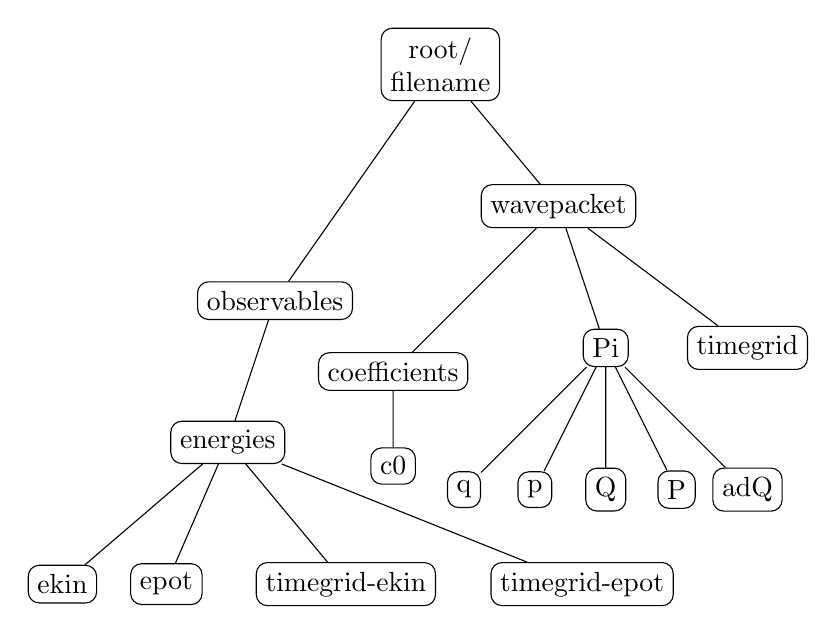
\begin{tikzpicture}[
baseline,
scale=1.2,
every node/.style = {shape=rectangle, rounded corners, draw, align=center},
]]
  \node {root/\\filename}
    child[yshift=-1cm,xshift=-1cm]
    {
    node{observables}
    child[xshift=-0.5cm]
            {
            node{energies}
    		child[xshift=0.5cm]{node{ekin}} 
    		child[xshift=0.1cm]{node{epot}}
    		child[xshift=0.5cm]{node{timegrid-ekin}}
    		child[xshift=1.5cm]{node{timegrid-epot}}
    		} 
    }
    child[xshift=0.5cm] 
    { 
    node {wavepacket}
    child[xshift=-0.25cm,yshift=-0.25cm]{node{coefficients}
    child[yshift=0.5cm]{node{c0}}}
    child[xshift=0.5cm]
    {
    node {Pi}
    child[xshift=1.5cm]{ node {q} }
    child[xshift=0.75cm] { node {p} }
    child { node {Q} }
    child[xshift=-0.75cm] { node {P} }
    child[xshift=-1.5cm] { node {adQ}}    
    }
    child[xshift=0.5cm]{node{timegrid}} 
	};
\end{tikzpicture}
}
\caption{Depiction of desired internal structure of a H5File}
\label{graph:file}
\end{figure}
To create a \textit{Group} only a \texttt{string} argument is required which acts as name but more importantly also as path similar to figure \ref{graph:file}. As previously indicated a \textit{H5File} has root \textit{Group} "/" by default after allocation. To accomplish the structure as in figure \ref{graph:file} the path is included in the name. For instance to have a \textit{Group} "wavepacket" after the root "/" and a \textit{Group} "Pi" after "wavepacket" the first name will be modified to "/wavepacket" and the second to "/wavepacket/Pi". This implies that every intermediate node in figure \ref{graph:file} will be a \textit{Group}. The leafs however will be \textit{DataSets} which will be explained in the next section \ref{seq:dataset}.

\section{DataSet}
\label{seq:dataset}
The constructor of the \textit{DataSet} class demands four arguments with individual type \textit{string}, \textit{DataType}, \textit{DataSpace} and \textit{DSetCreatPropList}. The first argument analogous to \textit{Group} is the name with its path included. For example the \textit{DataSet} "ekin" has the complete name "/observables/energies/ekin". As the name indicates the second and the third argument specifies the type and space of the data. Lastly the forth argument defines the properties at creation. This incorporates which data layout is chosen. The \textit{DataSet} has three types of layouts to store raw data. These are \texttt{H5D\_COMPACT}, \texttt{H5D\_CONTIGUOUS} and \texttt{H5D\_CHUNKED}. Figure \ref{fig:datalayout} should illustrate the inner workings of these layouts.

%\begin{figure}[ht!]
%\centering
%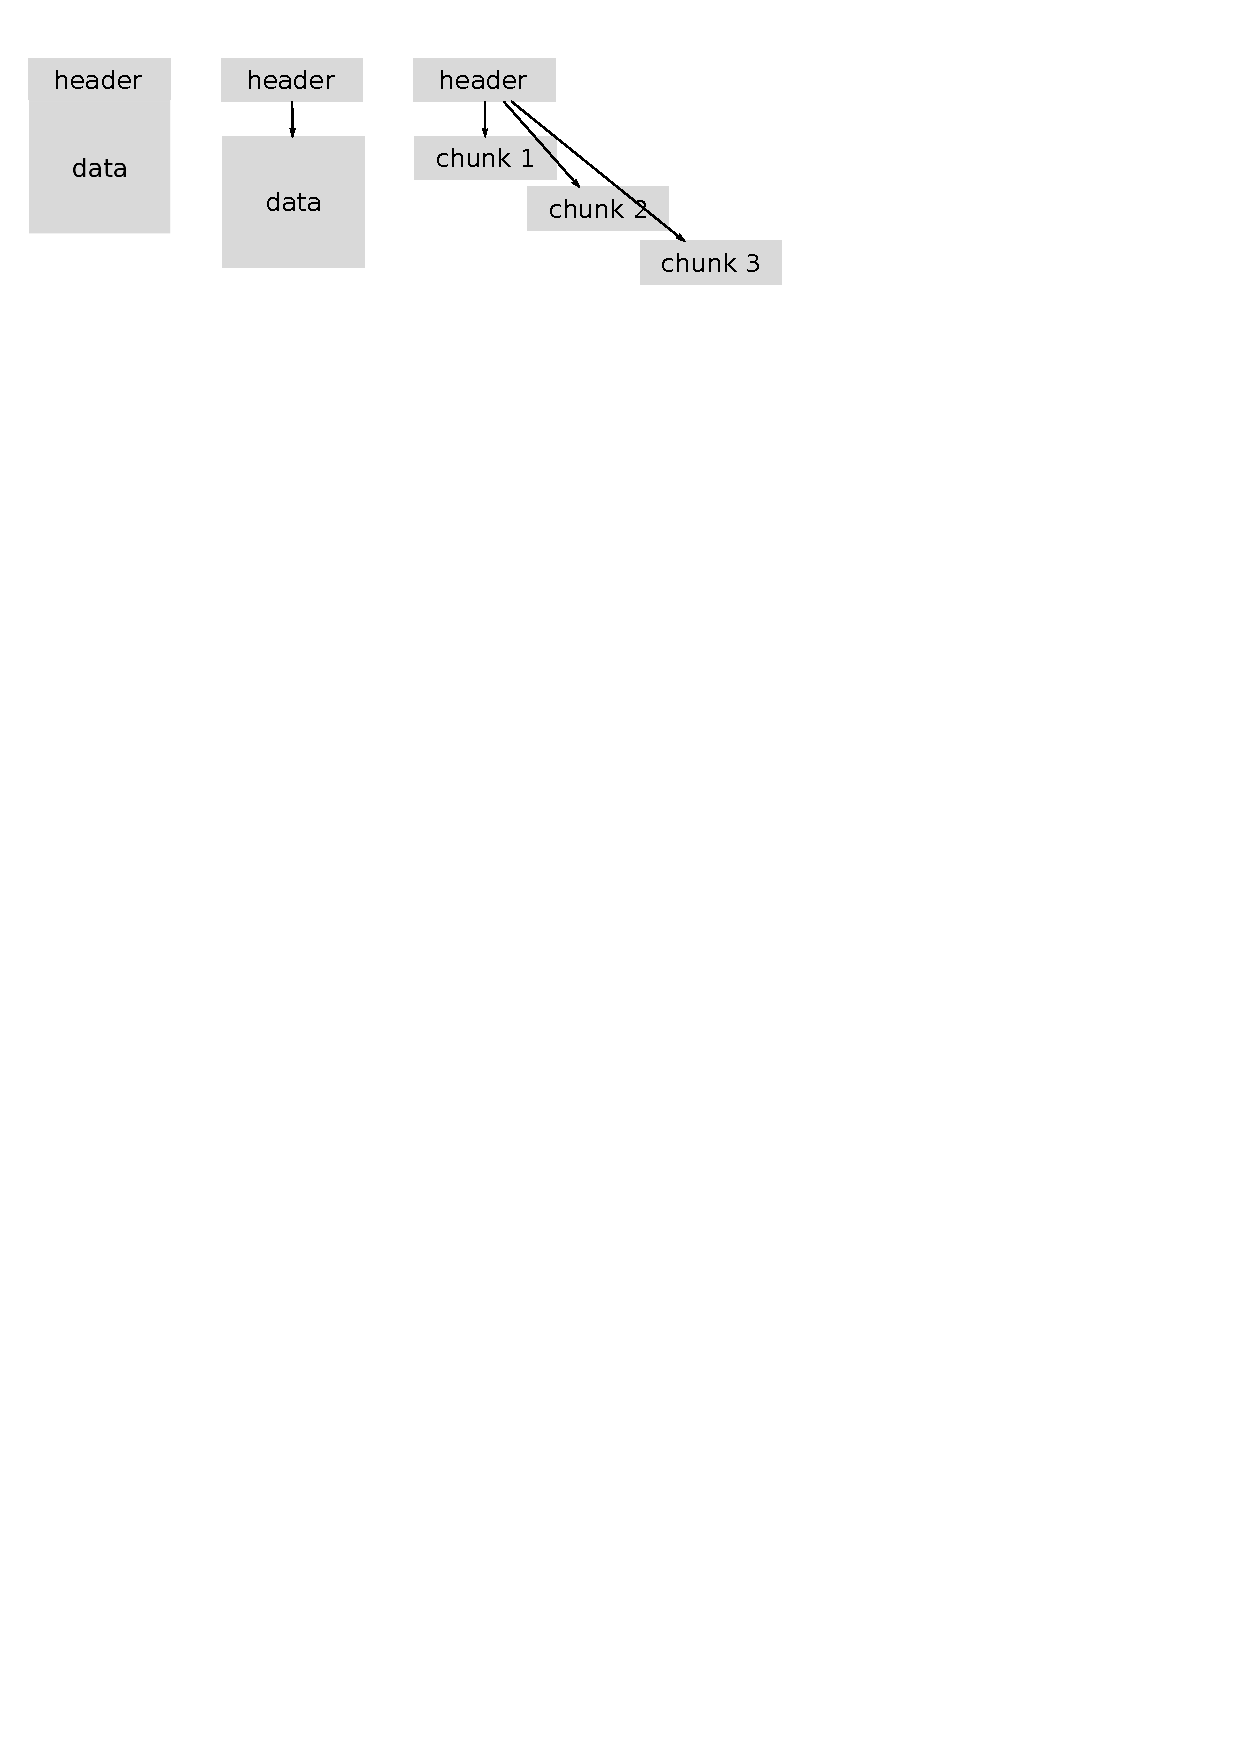
\includegraphics[width=\textwidth]{data_layout.pdf}
%caption{The three data layouts in \textit{DataSet}}
%\label{fig:datalayout}
%\end{figure}
\begin{figure}[ht!]
\resizebox{\textwidth}{!}{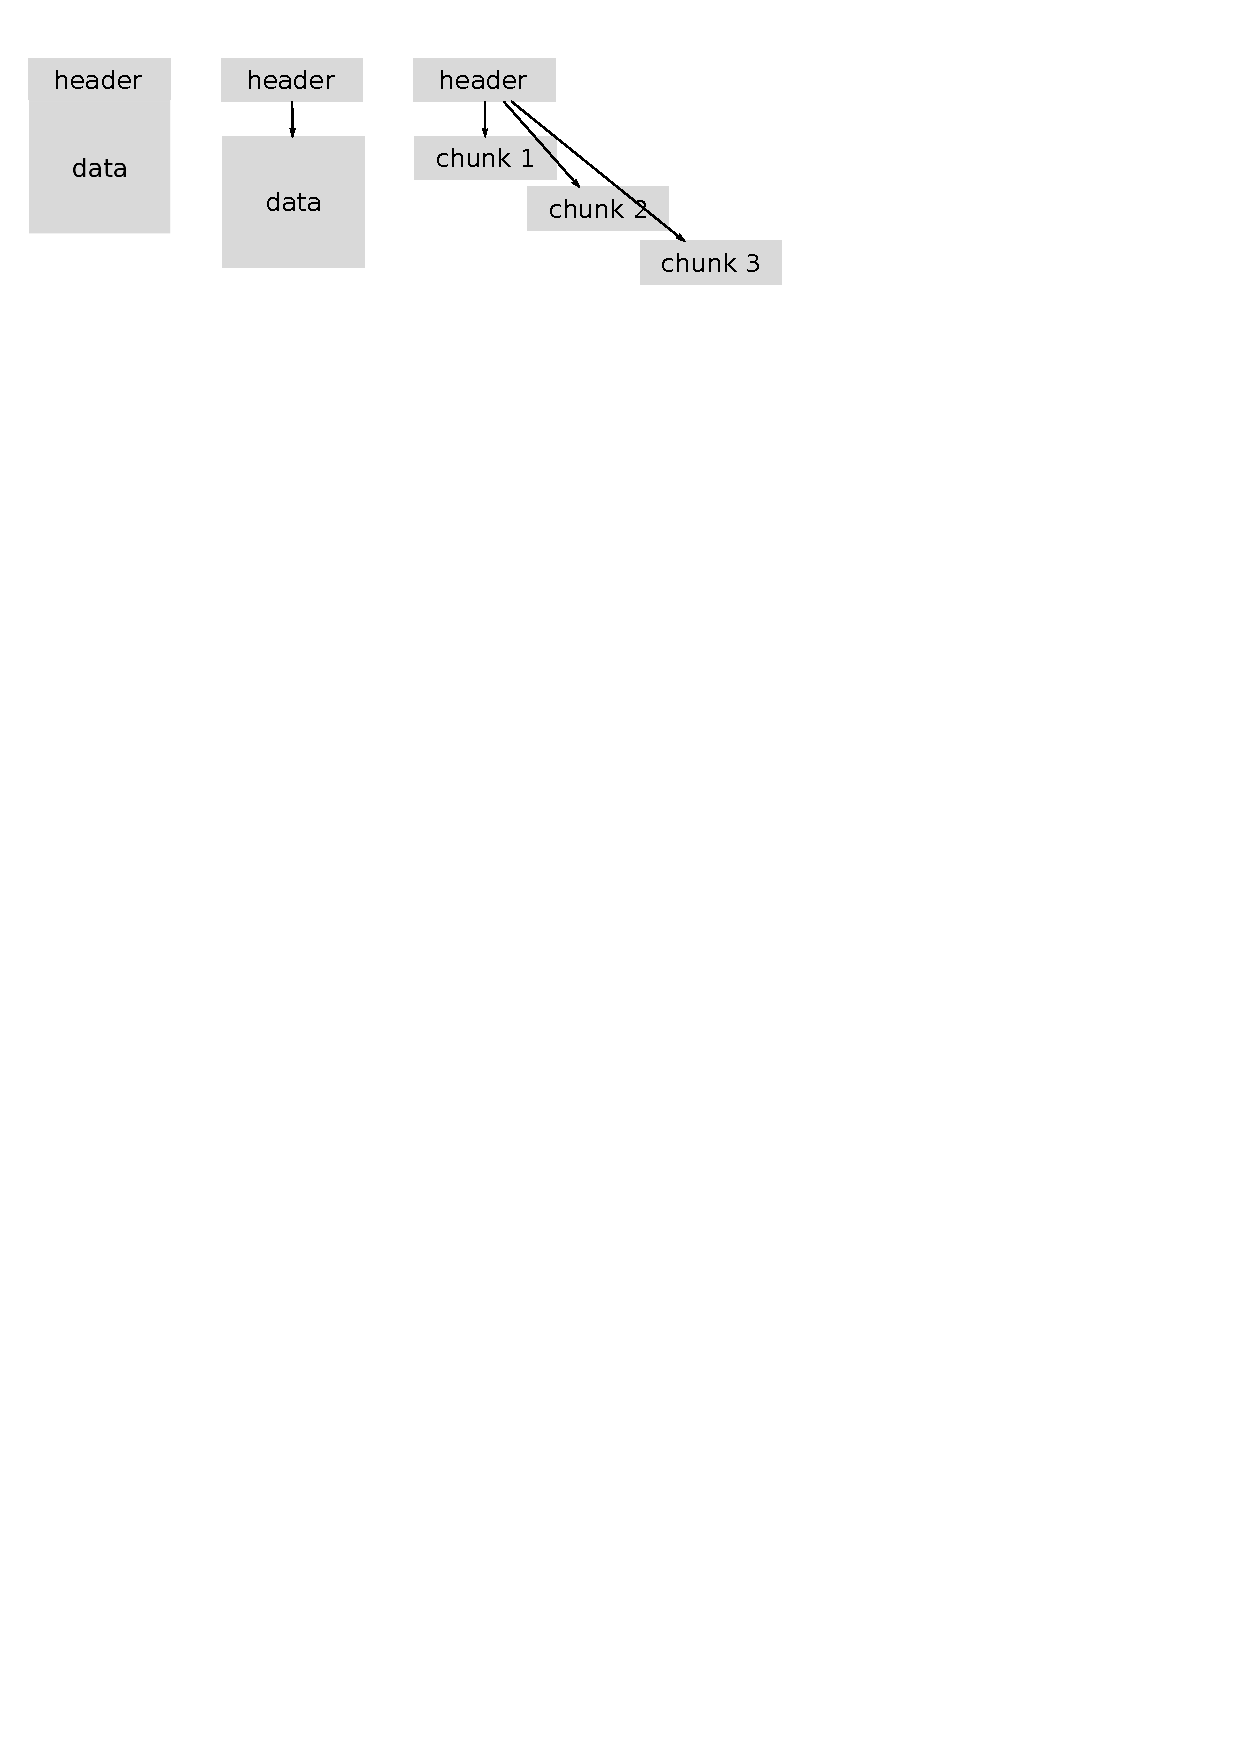
\includegraphics{data_layout.pdf}}
\caption{The three data layouts in \textit{DataSet}}
\label{fig:datalayout}
\end{figure}

If the data is sufficiently small \texttt{H5D\_COMPACT} will be used. In this layout the data address follows right after the header as shown on the left. When the data is bigger but still has a constant size \texttt{H5D\_CONTIGUOUS} is the right layout. This one allows that the address of the data can be arbitrary in memory and is saved in the header. The last layout \texttt{H5D\_CHUNKED} on the right is useful assuming the size of the data is unknown. The data will be divided continuously into chunks with constant size where the address will be saved in the header. This means when a chunk is full a new one gets allocated with its address saved into the header. As the perceptive reader can guess the last layout is of most relevance for this project. A simulation generates new data in each time step which in essence is ideal for the size of a chunk because it further allows to label each chunk to its corresponding time step. This will be later used to match data according to its time label.

\section{DataType}
The language C++ itself supports data types such as int, double, char etc. but these cannot be used directly in a binary data format.
This is caused by different data representation which are not homogeneous across different operating systems and system architectures. For example the difference between little-endian and big-endian machines. Thus the library has its own definitions which are compatible across platforms which are incorporated into the different classes seen in figure \ref{graph:hierarchy}. It is intuitively clear from their names which classes must be used to describe which data types. For instance for writing floating point numbers the \textit{FloatType} class is used. In this object further changes of characteristics can be done such as changing from default IEEE representation. In this project the \textit{PredType} and \textit{CompType} are of most relevance. The \textit{PredType} is predetermined meaning there is no explicit constructor needed. From this class \textit{NATIVE_INT} is used to write the respective time labels for the data. The \textit{CompType} class is utilized for writing complex numbers and also this class has to be explicit constructed which will be explained in section \ref{seq:datatypedec}.

\section{DataSpace}
To describe the dimensionality of our data the \textit{DataSpace} class is required. The construction of such a \textit{DataSpace} is straightforward. Firstly the library needs to know the number of dimensions of the desired space. Secondly it has know the number of elements in each dimension. For the second argument an array of \texttt{hsize\_t} is expected instead of \texttt{int} as described in section \ref{seq:internaltypes}. To give the reader an idea the following code depicts the \textit{DataSpace} of a time grid.

\begin{lstlisting}
int rank = 1;
hsize_t size[rank];
size[0]=number_of_timesteps;
DataSpace limited_timespace(rank,size);
\end{lstlisting}
The problem herein lies in the number of time steps which is known only at runtime but the constructor expects it at compiletime. This leads to another approach which is to define a unlimited \textit{DataSpace}. The library allows this if an additional optional argument is added. This argument has to be of the same data type as the second argument and contains the maximum size of each dimension. The library expects that this argument has to be greater or equal than the previous argument otherwise an exception is thrown. For an unlimited space a special state is used namely \texttt{H5S\_UNLIMITED}. The above example code changes to the following if an unlimited space is desired:
\begin{lstlisting}
int rank = 1;
hsize_t size[rank] = {1};
hsize_t maxsize[rank]={H5S_UNLIMITED};
DataSpace unlimited_timespace(rank,size,maxsize);
\end{lstlisting}

\section{PropList}
%%%
This class is used to create a new property as an instance of some property class. These constructed default classes are: \texttt{H5P\_FILE\_CREATE} for \textit{H5FILE} creation, \texttt{H5P\_FILE\_ACCESS} for \textit{H5FILE} access, \texttt{H5P\_DATASET\_CREATE} for \textit{DataSet} creation, \texttt{H5P\_DATASET\_XFER} for raw data transfer and \texttt{H5P\_MOUNT} for \textit{H5File} mounting.

\subsection{DSetCreatePropList}
This property list is used to change the mentioned data layout in figure \ref{fig:datalayout}. %We use a \textit{DSetCreatPropList} to change the properties of how raw data is organized on disk and how the raw data is compressed. 
When default constructed a \textit{DataSet} is simple meaning \texttt{H5D\_COMPACT} but this doesn't allow us easy extension of the \textit{DataSet}. For allowing unlimited extension we change the property of how raw data is organized by creating this property list and changing the chunk dimension to the time step size.

\section{Attribute}
An \textit{Attribute} is used to write additional information to an existing \textit{Group} or \textit{DataSet} to describe the nature and/or the intended usage or the object. To create an \textit{Attribute} it has to be attached to an extisting \textit{Group} or \textit{DataSet}. The creation is similar to a \textit{DataSet} because the same arguments are needed except for the \textit{DSetCreatPropList} only the \texttt{H5P\_DEFAULT} is allowed.


\chapter{Writer Template}

\section{DataType Declaration}
\label{seq:datatypedec}


\section{Setup write options}

\section{Setup write hierarchy}

\section{Prestructure}

\section{Selection}

\section{Transformation}

\section{Writing}

\section{Extension}

\section{Update}

\section{Poststructure}

\section{Inner workings in a picture}

\section{Usage in a simulation main file}


\chapter{Data Test}

\section{Introduction to GoogleTest}

\section{The Main C++ File}


\chapter{Conclusion}

